
\section{Hardware}
The system created in this thesis will be integrated into an existing driver cell model, which is shown im Figure \ref{fig:itiv-driver-cell} and thus has to fit certain constraints.


\subsection{Camera}

- Realsense
- Testrack


\section{Software}
In principle, it is possible to classify hand gestures directly from recorded depth information using machine learning. As in \cite{Molchanov2016}, a combination of a CNN and a downstream RNN can be used for this purpose. In this variant \todo{better formulation}, however, the structure of the network and the number and type of classes are strictly coupled. Adding, removing or changing a class would force us to retrain large parts of the network.
A further problem of this direct approach is that a sufficient amount of training data, consisting of image sequences and corresponding class labels, must be available for a reliable classification.

If new hand gestures with few example data are to be learned, and/or in the ideal case after unique Vormachen, it makes sense to divide the data processing into two sequential steps:

First, we generate a per-frame estimate of the current hand pose from the 2.5-dimensional input data (RGB-D). 


A possible time dependence of the respective hand gesture is not yet taken into account. 

\subsection{Input Format}
The camera used in this thesis, the Intel Realsense D435 provides multiple types of image streams:

\begin{itemize}
	\item An \textbf{RGB} Stream from a full HD RGB camera. 
	\item Two \textbf{infrared} image streams, provided by the two infrared modules and
	\item a \textbf{depth/disparity} map stream which is preprocessed by the camera and provides depth information with a 16 bit resolution.
\end{itemize}

For precise results it seems desirable to include all three types of input streams in the process of pose estimation in order to obtain a maximum amount of information. But in practice there are several limitations which restrict the use of the RGB and infrared streams.

Restrictions for the RGB input stream are mainly caused by the labeling process during dataset creation. Precise labeling of human hand pose datasets is impossible to achieve manually since single point of view (\markup{POV}\abbrev{POV}{Point Of View}) recordings of hand poses typically suffer from severe self-occlusion: Garcia-Hernando et al. \cite{GarciaHernando2017} count 10 occluded finger joints on average in their data set. In order to obtain reliable training data, Garcia-Hernando et al. use a body-attachable motion capturing (\markup{MoCap}\abbrev{MoCap}{Motion Capturing}) system which allows to automatically annotate the incoming image stream with precise pose information. 

While the pose information provided by this kind of automated pose annotation provides trustable pose information, it has the disadvantage that the used \markup{MoCap} system is clearly visible in the RGB images, as can be seen in Figure \ref{fig:garcia-rgb-problem}. The white cables and the tape used to fixate the sensors This bears the risk of the feature extractor overfitting on the high contrast extraneous features, rendering the trained network unusable for the intended use with bare hands. 

The infrared stream shares the same limitations but has the additional downside that to the best knowledge of the author no publicly available hand pose data set provides infrared images alongside their RGB-D data. 

The only remaining input image type is the depth map. Although the used \markup{MoCap} system might still be detectable in depth images, the contrast around the attached sensors is significantly reduced compared to the RGB images. Apart from this advantage, depth images are robust against sudden changes in illumination as long as the infrared images used to calculate the disparity are not overexposed. A third advantage that comes with disregarding RGB data is the reduced danger of overfitting on certain skin colors and thus creating a 'racist AI' \cite{Murray2019, Dietz2019, Solly2019} since depth maps provide no color information at all.

\begin{figure}
	\centering
	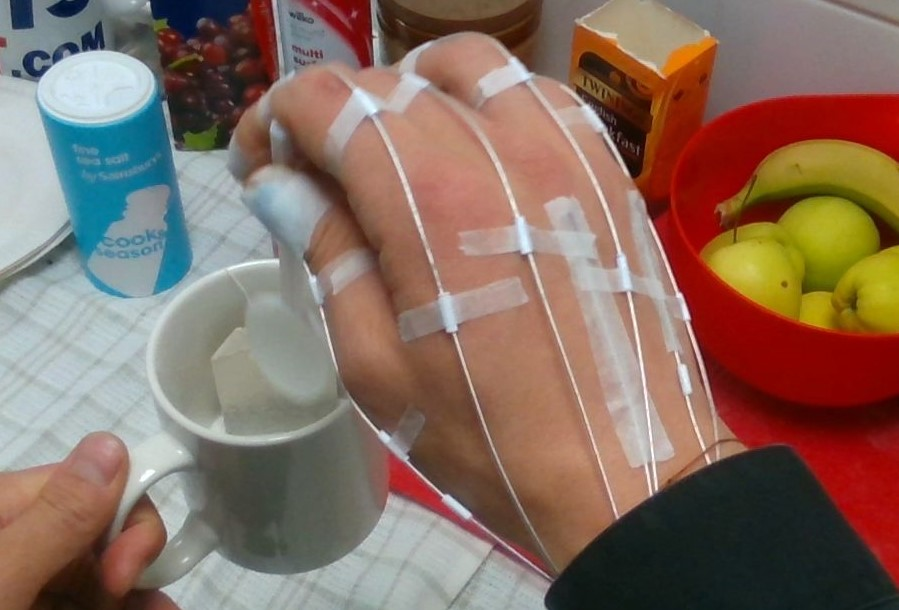
\includegraphics[width=0.7\linewidth]{Ressourcen/garcia-rgb-problem}
	\caption[Attachable motion tracking system]{Attachable motion tracking system in \cite{GarciaHernando2017}. \\ \textbf{Source:} \cite{GarciaHernando2017}}
	\label{fig:garcia-rgb-problem}
\end{figure}

\begin{figure}
	\centering
	\usetikzlibrary{arrows.meta}
\tikzset{%
	>={Latex[width=2mm,length=2mm]},
	% Specifications for style of nodes:
	base/.style = {rectangle, rounded corners, draw=black,
		minimum width=4cm, minimum height=1cm,
		text centered, font=\sffamily},
	activityStarts/.style = {base, fill=blue!30},
	startstop/.style = {base, fill=red!30},
	activityRuns/.style = {base, fill=green!30},
	process/.style = {base, minimum width=2.5cm, fill=orange!15,
		font=\ttfamily},
}
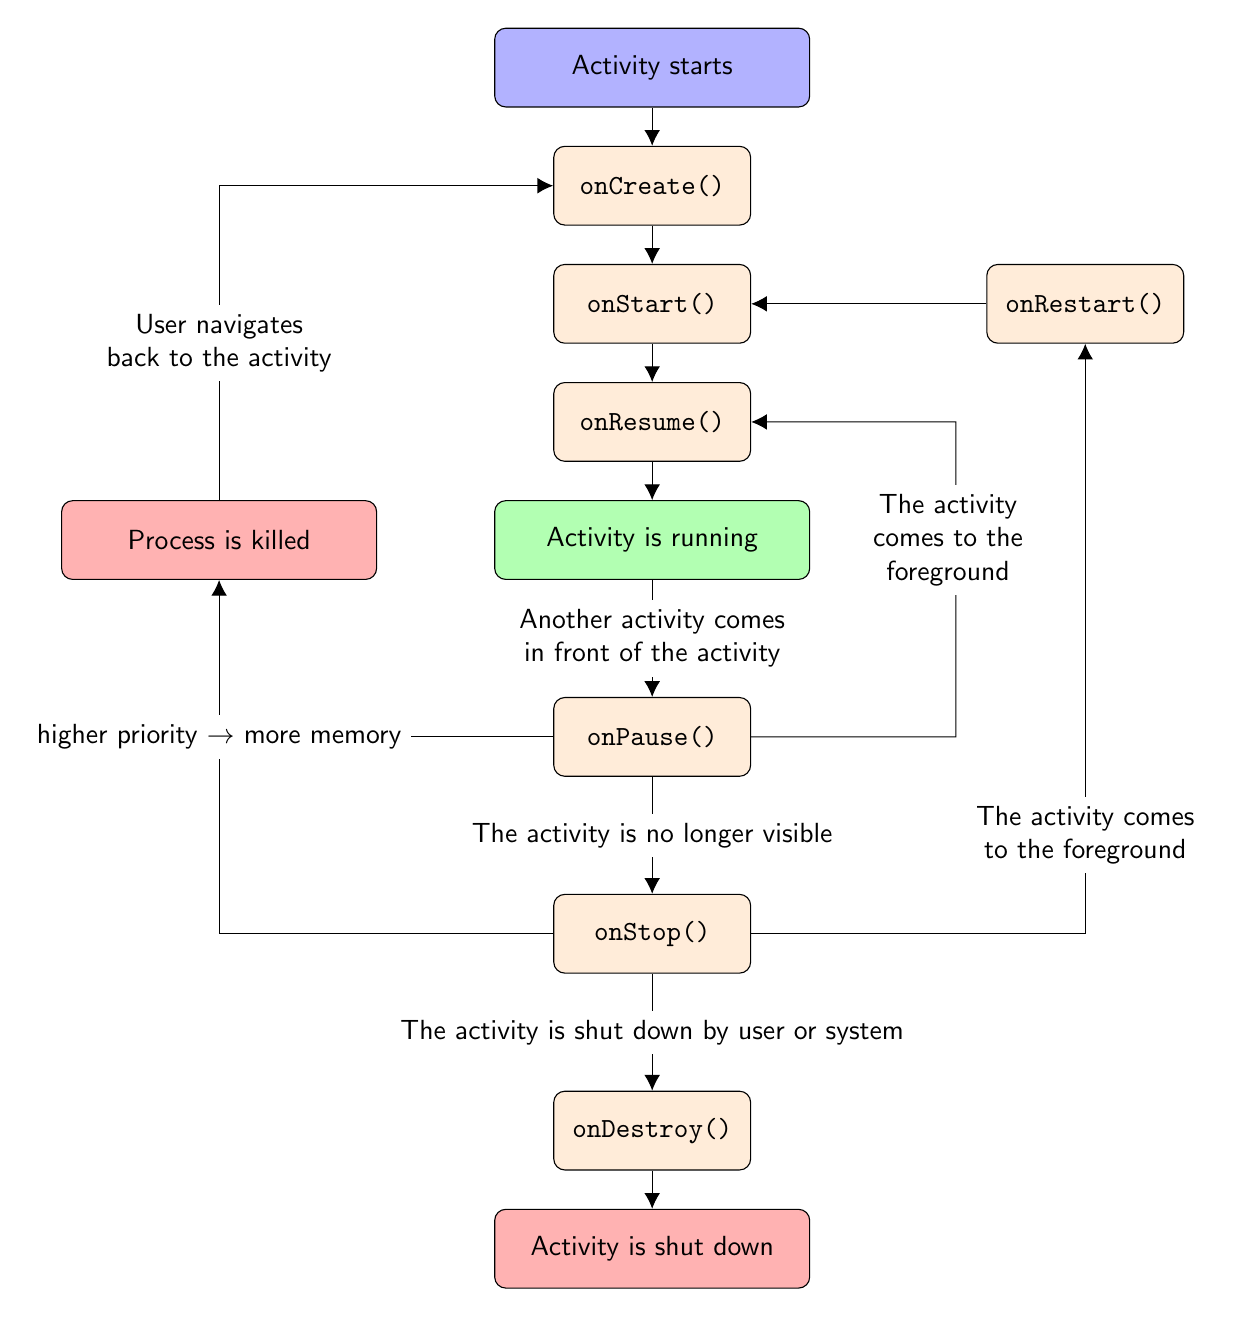
\begin{tikzpicture}[node distance=1.5cm,
    every node/.style={fill=white, font=\sffamily}, align=center]
  % Specification of nodes (position, etc.)
  \node (start)             [activityStarts]              {Activity starts};
  \node (onCreateBlock)     [process, below of=start]          {onCreate()};
  \node (onStartBlock)      [process, below of=onCreateBlock]   {onStart()};
  \node (onResumeBlock)     [process, below of=onStartBlock]   {onResume()};
  \node (activityRuns)      [activityRuns, below of=onResumeBlock]
                                                      {Activity is running};
  \node (onPauseBlock)      [process, below of=activityRuns, yshift=-1cm]
                                                                {onPause()};
  \node (onStopBlock)       [process, below of=onPauseBlock, yshift=-1cm]
                                                                 {onStop()};
  \node (onDestroyBlock)    [process, below of=onStopBlock, yshift=-1cm] 
                                                              {onDestroy()};
  \node (onRestartBlock)    [process, right of=onStartBlock, xshift=4cm]
                                                              {onRestart()};
  \node (ActivityEnds)      [startstop, left of=activityRuns, xshift=-4cm]
                                                        {Process is killed};
  \node (ActivityDestroyed) [startstop, below of=onDestroyBlock]
                                                    {Activity is shut down};     
  % Specification of lines between nodes specified above
  % with aditional nodes for description 
  \draw[->]             (start) -- (onCreateBlock);
  \draw[->]     (onCreateBlock) -- (onStartBlock);
  \draw[->]      (onStartBlock) -- (onResumeBlock);
  \draw[->]     (onResumeBlock) -- (activityRuns);
  \draw[->]      (activityRuns) -- node[text width=4cm]
                                   {Another activity comes in
                                    front of the activity} (onPauseBlock);
  \draw[->]      (onPauseBlock) -- node {The activity is no longer visible}
                                   (onStopBlock);
  \draw[->]       (onStopBlock) -- node {The activity is shut down by
                                   user or system} (onDestroyBlock);
  \draw[->]    (onRestartBlock) -- (onStartBlock);
  \draw[->]       (onStopBlock) -| node[yshift=1.25cm, text width=3cm]
                                   {The activity comes to the foreground}
                                   (onRestartBlock);
  \draw[->]    (onDestroyBlock) -- (ActivityDestroyed);
  \draw[->]      (onPauseBlock) -| node(priorityXMemory)
                                   {higher priority $\rightarrow$ more memory}
                                   (ActivityEnds);
  \draw           (onStopBlock) -| (priorityXMemory);
  \draw[->]     (ActivityEnds)  |- node [yshift=-2cm, text width=3.1cm]
                                    {User navigates back to the activity}
                                    (onCreateBlock);
  \draw[->] (onPauseBlock.east) -- ++(2.6,0) -- ++(0,2) -- ++(0,2) --                
     node[xshift=1.2cm,yshift=-1.5cm, text width=2.5cm]
     {The activity comes to the foreground}(onResumeBlock.east);
  \end{tikzpicture}
	\caption{}
	\label{fig:software-net-structure-blackbox}
\end{figure}

\subsection{Training}
	Aufgrund des zweistufigen Aufbaus kann auch das Training des Netzes in zwei Stufen erfolgen.



\section{Datasets and Data Generation}
